\chapter{Utveckling med Meteor av Johan Thornström}
\section{Introduktion}
\label{sec:johan_t-introduction}
Mjukvaruutveckling med hjälp av ramverk är något som kan spara tid i ett projekt. När en utvecklare i ett pågående projekt ska börja vidareutveckla den existerande kodbasen, behöver denna person sätta sig in i de mjukvarubibliotek som används. Utvecklaren behöver kunna förstå dessa bibliotek och hur de används inom kodbasen. Den tid som personen kräver för att sätta sig in i koden kan ta en längre tid än vad projektets tidsramar tillåter. Tanken med ett ramverk är att packetera de olika bibliotek som kan används tillsammans. Det innebär att ramverket gör att utvecklaren inte behöver oroa sig över vissa delar av funktionalitet och integration. Det går naturligtvis också att inte använda sig av ett ramverk. I vissa fall är det mer lämpligt då utvecklaren får mer kontroll och frihet. Man kan utveckla en mer robust applikation än vad ett ramverk tillåter. Kostnaden kan dock vara att det tar mer tid att utveckla om man inte är tidigare insatt i de miljöer som används. 
\subsection{Syfte}
\label{sec:johan_t-syfte}
Rapporten behandlar de utmaningar som finns gällande utveckling av applikationer i ett projekt med flera deltagare. Jämföra deltagarnas tidigare erfarenheter av utveckling i programmering mot webbapplikationer och de ramverk som används. Det är tänkt att man ska få en överblick hur det går att arbeta med ett tidigare okänt ramverk. Även hur ramverket påverkar gruppens möjlighet att skapa slutvärde för kund.
\subsection{Frågeställning}
\label{sec:johan_t-frågeställning}
I det här projektet har medlemmarna från grupp 2 i kursen TDDD96 använt sig av Meteor som är ett ramverk för utveckling av applikationer i JavaScript under våren 2017. Målet med denna undersökning är dels att undersöka användningen av ramverket Meteor för projektgruppen. Dessutom om hur det går att använda externa bibliotek när arbetet utförs under en kort tidsram. Frågeställningarna blir därmed.
\newpage
\begin{enumerate}
\item Vilka fördelar och nackdelar har ramverket Meteor för vårt kandidatprojekt?
\item Hur kan användning av externa bibliotek ha för inverkan på vårt kandidatprojekt?
\end{enumerate}
\section{Bakgrund}
\label{sec:johan_t-bakgrund}
När ett projekt ska utföras inom en tidsram så kan det finnas en risk att alla de krav från kravspecifikationen inte hinner uppfyllas. Detta kan bero på att projektgruppen inte har tidigare erfarenher men samtidigt vill komma igång så fort som möjligt och att implementeringstiden ska bli så kort som möjligt. Om den projektgruppen har varierande erfarenhet av utveckling finns risken att det blir stor variation i hur mycket varje medlem i projektgruppen bidrar. Då bör man ha en tydlig dokumentation och klara riktlinjer, så att hela projektgruppen snabbt kan börja bidra. Ett ramverk som Meteor bidrar med bra riktlinjer för hur implementering kan ske, så att en utvecklare med bristande tidigare kunskap snabbt kan komma igång med utvecklingen. Detta gör att utvecklaren snabbt kan börja bidra till projektet så tidigt som möjligt. 
\\ \\ 
I det här projektets fall så har gruppen utgått från ett givet ramverk som ingen hade tidigare erfarenhet av. Endast några hade över huvudtaget någon erfarenhet av utveckling av webbapplikationer. Dessutom så har kursens ett fokus på dokumentation vilket begränsar den tid som kan läggas på utveckling ännu mer. Den inlärningstid som krävs blir lång oavsett hur mycket tid som varje projektmedlem förväntas lägga. I vårt fall betyder det att den tid projektmedlemmarna spenderar på utveckling helst ska bli så pass effektiv som möjligt om man ska kunna uppfylla så många krav från kravspecifikationen som möjligt.
\section{Teori}
\label{sec:johan_t-teori}
I denna del kommer teori relaterat till Meteor och Node.js att behandlas. Mer utförlig bakgrundsinformation finns om Meteor vid kapitel \ref{subsec:meteor} och till Node.js vid \ref{subsec:node}. Den information som behandlas här är hämtat från respektive systems hemsidor.
\subsection{Meteor}
\label{sec:johan_t-meteor}
Meteor är utvecklat av Meteor Development Group och släpptes för allmänheten 2012 och har varit under ständigt förändring sedan dess. Ett av de mål Meteor hade från början var att man snabbt skulle kunna installera Meteor och producera en fungerande prototyp inom loppet av en helg. Nedan presenteras de sju principer Meteor Development Group använde sig av när de introducerade Meteor i slutet av 2011.\cite{website:oldmeteor}
\begin{enumerate}
\item Istället för att skicka HTML-kod över nätverket, skicka data och låt klienten avgöra hur det ska visas.
\item Ett språk. Skriv kod för både klient och server i samma utvecklignsmiljö för JavaScript
\item Databas överallt. Använd samma transparenta API för att få tillgång till din databas från klient eller server.
\item Fördröjningskompensation. På klienten, använd förhämtning och modellsimulering för att det ska se ut som det inte är fördröjning att anropa databasen.
\item Reaktiv helhetslösning. Uppdaterar i realtil, klint till databas ska ha en händelsedrivet gränssnitt tillgängligt.
\item Ett ekosystem. Meteor har öppen källkod och intregerar, istället för att ersätta existerande verktyg och ramverk.
\item Enkelhet motsvarar produktivitet. Att få något att se enkelt ut är att faktiskt göra det enkelt med hjälp av ett enkelt API.
\end{enumerate}
\subsection{Node Package Manager}
\label{subsec:johan_t-npm}
Meteors server är baserat på Node.js som är en exekveringsmiljö där Node Package Manager(npm) är dess pakethanteringssystem. Det pakethanteringssystemet uppfyller två funktioner. Ett är att förvara paket och moduler till Node.js som finns i en sökbar databas på deras hemsida. Där kan användarna själva ladda upp eller ladda ner paket och moduler. Det andra är att via terminalkommandon kunna ladda ner och installera moduler eller paket i sitt lokala program för Node.js.
\section{Metod}
\label{sec:johan_t-metod}
För att kunna få fram ett svar på frågeställningen om Meteors fördelar och nackdelar kommer de erfarenheter som gruppen har varit med om vara i åtanke. Under våren har gruppen fått sätta sig in i applikationen som är utvecklat i ramverket Meteor för att senare vidareutveckla det. Under projektets gång har diskussioner om fördelar och nackdelar dykt upp inom gruppen. Dessa diskussioner har projektgruppen haft under möten, i konversationer via vår interna Slack-grupp eller intern dokumentation. 
\\ \\
Angående användandet av externa bibliotek kommer främst att baseras på de erfarenheter projektgruppen har upplevt under projektets gång. Projektgruppen har suttit och utvecklat främst genom parprogrammering eller självständigt. Vid slutet av projektets tid var det runt 30 filer med över tre tusen rader kod som tagits fram.
\section{Resultat}
\label{sec:johan_t-resultat}
I detta kapitel presenteras resultatet på de frågställningar som har tagits fram. Eftersom båda frågeställningarna har två delfrågor så presenteras de separat. 
\subsection{Meteors fördelar}
I denna del presenteras de fördelar med Meteor som kommit fram under projektets gång.
\label{subsec:johan_t-meteor_fördelar}
\begin{figure}[h]
    \centering
    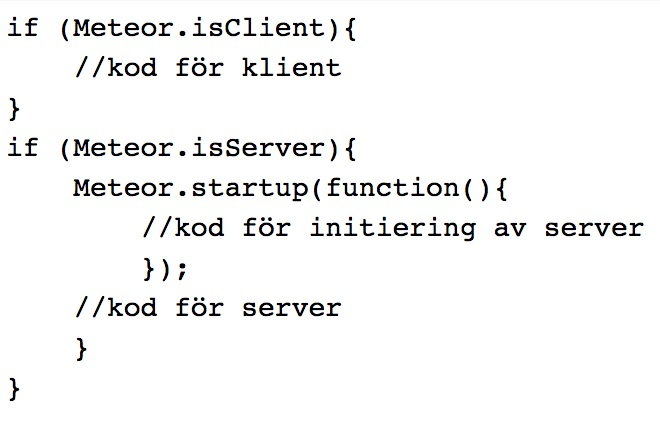
\includegraphics[scale=0.25]{Meteorexempelkod}
    \caption{Syntax för klient och server i Meteor.}
    \label{fig:meteor_syntax}
\end{figure}
\\
Om man så skulle vilja så kan man sköta all form av tänkbara beräkningar i både klient och server i samma js-fil. Hur man skiljer på en server och klient i Meteor kan man se i figur \ref{fig:meteor_syntax}. Man behöver inte skriva någon synkroniseringskod mellan server och klient. Första raden i dokumentet initieras en databas till projektet. Man kan alltså från klienten lägga till eller hämta data från databasen.
\\ \\
Eftersom Meteor använder sig av Node.js så kan man använda dess pakethanterare npm. En stor fördel med att ha tillgång till den pakethanteraren är att man enkelt kan hämta ner och installera externa bibliotek från Nodes hemsida. En stor fördel med att servern använder sig av JavaScript gör att man endast behöver ett språk för utveckling av klient och server. Tiden det skulle ta för en utvecklare att sätta sig in i flera språk istället för ett minskar inlärningstiden avsevärt.
\\ \\
I  projektet ska projektgruppen visualisera stora mängder Eiffelhändelser. De Eiffelhändelser som ska visualiseras har formatet JSON och det finns en stor mängd av olika typer av data. De datatyperna har även olika innerhåll vilket skulle försvåra förvaringen i en relationsdatabas. MongoDB som är Meteors databaslösning är en dokumentdatabas och sparar data i  BSON-format som betyder binary JSON. Skillnaden mellan JSON och BSON är att sökhastighet och lagringstorlek blir effektivare. Eftersom Eiffelhändelserna har ett likt format som databasen gör att prestandan ökar, dessutom att databasen endast behöver göra ett anrop för att hämta en specifik Eiffelhändelse när en relationsdatabas behöver flera. 
\subsection{Meteors nackdelar}
\label{subsec:johan_t-meteor_nackdelar}
Meteor sköter som nämnt i avsnitt \ref{subsec:johan_t-meteor_fördelar} synkroniseringen mellan klient och server. Den kod projektgruppen har tog fram körs alltså via Meteors egna syntax för JavaScript. Fördelen med att snabbt komma igång med utveckling skapar nackdelen att man förlorar kontrollen över hur applikationen körs. 
\\ \\
Att använda samma programmeringsspråk på både klient och server kan skapa abstraktionsproblem. Som man kan se i figur \ref{fig:meteor_syntax} så går det att inom samma fil göra beräkningar på både klient och server. Det går dessutom att anropa databasen utan att gå igenom servern vilket kan försvåra för en utvecklare att se förhållanden mellan olika moduler. 
\\ \\
Eftersom Meteor kommer med en specifik exekveringsmiljö och databas blir man låst till dessa. Skulle man utveckla en applikation som till exempel använder relationsbaserad data blir MongoDB ett suboptimal lösning. Eftersom Node.js kör JavaScript som är enkeltrådad så har man även problemet med skalbarhet. 
\subsection{Användning av externa bibliotek}
\label{subsec:johan_t-bibliotek}
Den stora vinsten med att använda sig av externa bibliotek är den den tid som sparades genom inte behöva implementera tidskrävande funktionalitet från grunden. Tack vare pakethanteraren går processen att ladda ner och installera de biblioteken fort. De externa biblioteken kan vara väldigt ambitiösa projekt vilket gör att man enkelt kan få en väldigt snygg lösning på funktionalitet i sin egna applikation.
\\ \\
Om man använder sig av ett externt bibliotek som har den funktionalitet som man vill ha fast med ett undantag kan man stå inför valet att förlora funktionalitet för att vinna tid.
\section{Diskussion}
\label{sec:johan_t-diskussion}
Projektgruppen skulle utveckla en prototyp där det var fokus på många olika funktionaliteter. När det är stor variation på funktionalitet som ska implementeras blir användandet av externa bibliotek ett bra verktyg då det kan finnas ett som uppfyller de funktioner som en funktion förväntas göra. Dessutom slipper utvecklaren att göra all funktionalitet från grunden.
\\ \\
Om man tittar på listan av principer som Meteor följde vid starten som kan ses vid avsnitt \ref{sec:johan_t-meteor} så sammanfattar punkt sju målet med Meteor väl. Enkelhet motsvarar produktivitet. Man ska snabbt kunna komma igång och producera en prototyp under kort tid. Det är möjligt tack vare att ramverket sköter många av de vitala delarna en applikation. På deras hemsida är bland det första man ser följande citat.\cite{website:meteor}
\begin{itemize}
\item Få ut mer av mindre kod - Utför med 10 rader kod vad annars skulle ta 1000, tack vare en integrerad JavaScript-stack som sträcker sig från databasen till användarens skärm
\end{itemize}
Ramverket sköter kommunikationen mellan klient och server så utvecklaren inte behöver tänka på det. Robustheten går att ifrågasätta om man skulle arbete i ett störra projekt under en längre tid om man låter ramverket sköta vitala delar åt en. Eftersom ramverket sköter väsentliga delar av funktionaliteten kan man inte garantera att koden uppfyller de krav man kan ställa. Sedan är Node.js relativt nytt och det finns inga tydliga riktlinjer för arkitektur eller implementering.\cite{review_node} Att designa specifika system blir därmed lätt komplext och svårt att underhålla. Vid saknad av riktlinjer blir tid för till och med installation av arbetsmiljön ett problem. Sedan när Meteor är byggt som ett lager ovanpå Node.js så blir det ytterligare ett lager av komplexitet vid hantering av exekveringsmiljön.
\\ \\
En nackdel med att jobba med ett ramverk som Meteor blir att man blir begränsad att jobba inom det ramverket. I vårt fall som jobbar under kort tid med implementering och har en databas med JSON-objekt blir Metoer ett bra val då databaslösnignen är väl lämpad för den typen av data. Sen att Meteor sköter all hantering av synkronisering mellan klient, server och databas minskar tiden att förstå fundamentala principer med Node.js. Skulle projektgruppens medlemmar börja jobba med Node.js eller MongoDB efter projektet men utan Meteor så skulle det blir en ny upplärningsprocess då Meteor har sitt egna syntax på hur en utvecklare anropar klient eller server.
\\ \\
Att använda samma programmeringsspråk på både klient och server kan skapa förvirring. När kod hos klienten kan göra anrop till databasen utan att behöva gå igenom servern uppstår abstraktionsproblem. I vårt fall så är det ett stort fokus på visualisering av data vilket gör att man skulle vilja ha en tydlig separation av klient och server så man enkelt kan lägga funktionalitet för rending på klienten.
\\ \\
I en kurs som den här, ett kandidatarbete där fokuset är på dokumentation blir ett ramverk som Meteor en bra lösning. Eftersom ramverket ger en bra grund för en utvecklare utan tidigare erfarenheter att snabbt kunna skapa något som kommer att ge värde till kund. Nackdelen är att man blir låst i hur Meteor och när det är ett ramverk som ständigt är under utveckling och ett api som förändras ofta får man begränsad kunskap om webbprogrammering. Men eftersom det är inte det huvudsakliga syftet med kursen är det ett överkomligt problem.
\section{Slutsats}
\label{subsec:johan_t-slutsats}
Att använda ramverket Meteor i vårt syfte var ett bra val. Meteor gjorde att vi snabbt kunde komma igång och utveckla applikationen. Användning av externa bibliotek gjorde att vi inte behövde lägga ner mycket tid på funktionalitet som redan fanns tillgängligt Eftersom målet med projektet främst var att visa upp olika funktionalitet som finns inom visualisering av kontinuerlig integration. På grund av den tidsbegränsning vi haft för implementering gjorde att användning av ramverk och externa bibliotek ett utmärkt val.